\documentclass[a4paper, fontsize=11pt, headsepline]{scrreprt}
\usepackage{scrlayer-scrpage}
\automark[chapter]{chapter}
\pagestyle{plain}
\usepackage{mathtools}
\usepackage{fontspec}
\defaultfontfeatures{Ligatures=TeX, Scale=MatchLowercase}
\newcommand{\euro}{€}
\usepackage[usenames, dvipsnames]{xcolor}
\usepackage{polyglossia}
\setdefaultlanguage[spelling=new]{german}
\setotherlanguage[variant=british]{english}
\usepackage{csquotes}
\usepackage[backend=biber, style=iso-authoryear]{biblatex}
\addbibresource{bib/main.bib}
\usepackage[section]{placeins}
\usepackage{minted}
\renewcommand{\listoflistingscaption}{Quellcodeverzeichnis}
\usepackage{longtable, booktabs}
\usepackage{graphicx, grffile}
\usepackage[pdfencoding=unicode, pdftitle={Evaluation aktueller Bibliotheken für Stream Graph Processing},
pdfauthor={Mirko Lelansky}, pdfkeywords={{Graph}, {Stream Processing}, {Integration}, {Apache Flink}},
citecolor=black, colorlinks=true, linkcolor=black, unicode=true, urlcolor=black]{hyperref}
\usepackage[acronym, toc]{glossaries}
\newglossaryentry{ACID}{name={Atomicity, Consistency, Isolation and Durability},
description={ACID steht für Atomarität, Konsistenz, Isolation und
Dauerhaftigkeit. Atomarität meint in diesem Zusammenhang, das eine Liste
von Operationen entweder vollständig oder gar nicht durchgeführt wird. Konsistenz
meint die Eigenschaft, dass die Datenbank sich nach einer Liste von Operationen
wieder in einem konsistenten Zustand befindet, wenn sie voher sich in einem
konsistenten Zustand befand. Isolation meint die Fähigkeit, das es keine
unkontrollierten Operationen auf den Daten gibt durch zwei parallele Prozesse.
Die Dauerhaftigkeit sagt aus, dass geschriebene Daten auch nach einem Ausfall
des Systems noch dauerhaft vorhanden sind.}}
\newacronym{API}{API}{Application Programming Interface}
\newglossaryentry{BASE}{name={Basically Available, Soft State,
Eventually Consistent}, description={BASE ist der Gegenpart zu \gls{ACID} für
NoSql-Systeme. Bei BASE geht es darum die Konsistenz der Verfügbarkeit
unterzuordnen, da es in verteilten Datenbanken nicht möglicht ist mit ACID die
geforderte Verfügbarkeit zu gewährleisten. Ein System, das nach BASE arbeitet
muss dabei immer die Verfügbarkeit vom \gls{CAP}-Theorem sicherstellen.
Soft States bedeutet, dass sich verschiedene Versionen eines Datenbestandes auf
dem einzelnen Knoten eines Clusters befinden können und nach einer gewissen Zeit
auf allen Knoten die letzte Version vorhanden ist und das System sich dann
wieder im Hard State befindet. Eventually Consistent meint, dass das System
nach einer gewissen Zeit sich wieder in einem konsistenten Zustand befindet.}}
\newglossaryentry{BigData}{name={BigData}, description={Der Begriff BigData
bezeichnet eine Datenmenge, die mit herkormlichen Mitteln nicht verarbeitet
werden kann, weil sie zu groß, zu unstrukturiert, zu komplex sind oder in
Echtzeit verarbeitet werden müssen. Dies hängt mit den \gls{5V's} zusammen.}}
\newglossaryentry{CAP}{name={Consistency, Availability, Partition Tolerance},
description={CAP steht für Konsistenz, Verfügbarkeit und Ausfalltoleranz und ist
ein Theorem für verteielte Systeme von Eric Brewer. Das Theorem sagt aus, dass
man lediglich zwei der drei Eigenschaften gleichzeitig einhalten kann, die
dritte wird man nie einhalten können. Verfügbarkeit ist dabei die Antwortzeit
eines Systems auf eine Anfrage. Konsistenz meint hierbei, dass nach einer
Änderung der Daten auf einem Knoten, diese an die anderen Knoten weitergereicht
wird. Ausfalltoleranz meint, dass das System auch bei Verlust von Nachrichten
noch weiterarbeit. \cite{Brewer2000}}}
\newacronym{CRUD}{CRUD}{Create, Read, Update and Delete}
\newglossaryentry{5V's}{name={5V's}, description={Die 5V's stehen für Volume,
Velocity, Variaty, Value und Validaty. Dabei steht Volume für die Datenmenge,
Velocity für Zeit mit der die Daten verarbeitet werden müssen, Variaty steht
für die Struktur der Daten, Value steht für den zu erzeugenden Mehrwert und
Validaty steht für die Datenqualität.}}

\makeglossaries
\setlength{\parskip}{\medskipamount}
%% Deutsche Kurzfassung und englisches Abstract auf eine Seite
\renewenvironment{abstract}{
    \begin{center}
    \normalfont\sectfont\nobreak\abstractname
    \end{center}
}{
    \par
}
\begin{document}
\pagenumbering{roman}
\begin{titlepage}
\begin{center}

\includegraphics[scale=1.5]{../material/images/THB_Logo.pdf} 
\vspace{0.5cm} 

\textbf{\begin{Large}
Fachbereich Informatik und Medien
\end{Large}}
\vspace{1cm}

\textbf{\begin{Huge}Masterarbeit\end{Huge}}
\vspace{0.5cm}

\begin{Large}
Evaluation aktueller Bibliotheken für Stream Graph Processing
\end{Large}
\vspace{2cm}

\begin{tabular}{rl}
Vorgelegt von: & Mirko Lelansky\tabularnewline
am: & 30.01.2019
\end{tabular}
\vspace{1cm}

zum Erlangen des akademischen Grades
\vspace{1cm}

\textbf{\begin{LARGE}MASTER OF SCIENCE\end{LARGE}}\\
\textbf{\begin{Large}(M.Sc.)\end{Large}}
\vspace{2cm}

\begin{tabular}{rl}
Erstbetreuer: & Prof. Dr.-Ing. Sven Buchholz\tabularnewline
Zweitbetreuer: & Prof. Dr.-Ing. Susanne Busse
\end{tabular}

\end{center}
\end{titlepage}

\begin{center}
\textsf{\textbf{\begin{Large}Selbstständigkeitserklärung\end{Large}}}
\end{center}

\noindent
Hiermit erkläre ich, dass ich die vorliegende Arbeit zum Thema

\smallskip{}

\noindent
\begin{center}
\textsf{Evaluation aktueller Bibliotheken für Stream Graph Processing}
\par
\end{center}

\smallskip{}

\noindent
vollkommen selbständig verfasst und keine anderen als die angegebenen Quellen
und Hilfsmittel benutzt sowie Zitate kenntlich gemacht habe. Die Arbeit wurde
in dieser oder ähnlicher Form noch keiner anderen Prüfungsbehörde vorgelegt.

\medskip
\noindent
Brandenburg/Havel, den %Datum

\vspace{1.7cm}
\noindent
Unterschrift

\begin{center}
\textsf{\textbf{\begin{Large}Danksagung\end{Large}}}
\end{center}

Hiermit möchte ich mich bei allen bedanken, die mich bei der Anfertigung dieser
Arbeit unterstützt haben. Mein besonderer Dank gilt meinen beiden
Betreuern Prof. Dr.-Ing Sven Buchholz und Prof. Dr.-Ing. Susanne Busse. Außerdem
möchte ich meiner Familie danken, die mich während meiner Studienzeit immer
tatkräftig unterstützt hat.

\begin{abstract}
Die Arbeit beschäftigt sich mit dem Thema \enquote{Stream-Processing} von
Graphen. Ziel der Arbeit ist es die gewählten Bibliotheken hinsichtlich ihrer
Funktionalität zu analysieren. Des Weiteren sollen die praktischen Möglichkeiten
ermittelt werden.

Dazu wird in den ersten Kapiteln die Theorie für die einzelnen Aspekte gelegt.
Dabei wird zuerst die Datenstruktur eines Graphen erläutert. Anschließend wird
das Konzept \enquote{Stream-Processing} vorgestellt. Abschließend werden die
einzelnen Bibliotheken vorgestellt und miteinander verglichen.

Nachdem die theoretischen Grundlagen gelegt wurden, wird das praktische Beispiel
erläutert und für die jeweiligen Bibliotheken ein Konzept entworfen und diesen
anschließend praktisch umgesetzt.

Abschließend erfolgt eine Zusammenfassung der Arbeit und ein Ausblick auf die
möglichen nächsten Schritte.
\end{abstract}

\begin{english}
    \begin{abstract}
        The topic of the thesis is \enquote{Stream-Processing} of graphs.
        The goal of the thesis is to analyses the functionality of the selected
        libraries. That includes the research of how useable they are in practice.
        
        In the first chapters the theory for every aspect will be explained.
        First the graph datastructure is described. After that the concept and
        methods of \enquote{Stream-Processing} are explained. At the end of
        chapter the different libraries are presented and compared.
        
        After the theory, the practical example is explained. That means that
        for every library a design is created and implemented.
        
        At the end of the thesis the summary of the work and a preview of the
        next possible steps are described.
    \end{abstract}
\end{english}

\tableofcontents
\clearpage
\pagenumbering{arabic}
\pagestyle{scrheadings}
\clearpairofpagestyles
\ihead{
\includegraphics[scale=0.5]{../material/images/THB_Logo_grey.pdf}}
\ohead{\headmark}
\cfoot[\pagemark]{\pagemark}
\printglossary[type=acronym, title=Abkürzungsverzeichnis, toctitle=Abkürzungsverzeichnis]
\chapter{Einleitung}
Durch den stetigen Fortschritt und der steigenden Komplexität der Anwendungen,
werden immer größere Datenmengen erzeugt. Sei es im privaten Umfeld durch die
Benutzung von Social-Media Platformen wie Facebook, Twitter,~\dots~oder im
gewerblichen Umfeld durch medinische Daten, Börsendaten,~\dots . Durch die
stetige Vernetzung von Alltagsgegenständen, welches man unter dem Begriff
IoT\footnote{Internet of the Things} zusammenfassen kann, stiegen diese
Datenmengen nochmals sehr stark an. Dies hat zur Folge, dass die Verarbeitung
dieser Datenmengen immer komplexer wird und dies mit nur einem einzelnen Rechner
nicht mehr möglich ist. Dies wird als \gls{BigData} bezeichnet. Bei der
Verarbeitung von großen Datenmengen wird zwischen zwei unterschiedlichen Methoden
unterschieden Batch-Processing und Stream-Processing. Beim Batch-Processing wird
eine feste Datenmenge in kleinere Einheiten unterteilt. Diese Teildaten werden
dann von mehreren Rechnern einzeln bearbeitet und anschließen die Ergebnisse
wieder kombiniert. Beim Stream-Processing gibt es keine feste Menge, sondern
die Daten kommen kontinuierlich in die Verarbeitung. Dadurch ist es möglich die
Daten in Echtzeit zu verarbeiten. Stream-Processing eignet sich für folgende
Einsatzgebiete:

\begin{itemize}
\item Fehlererkennung zum Beispiel bei Kreditkarten
\item Spracherkennung
\item Log-Analysen
\item Event-Verarbeitung
\end{itemize}

\begin{figure}
\centering
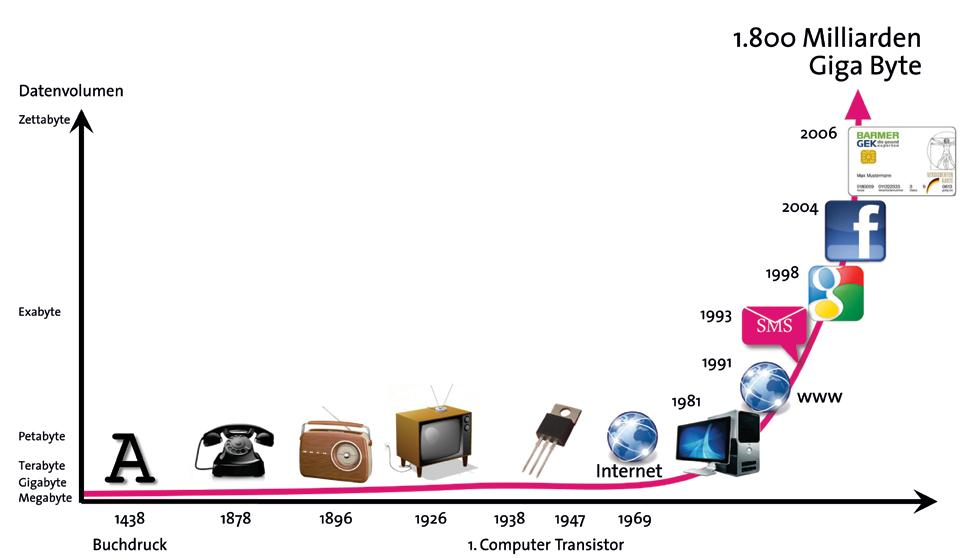
\includegraphics[scale=0.375]{../material/images/bitkom-lf-bigdata-2012-data_grow.jpg}
\caption{Erhöhung der Datenmenge von 1400 bis 2006 \parencite{Weber2012}}
\label{fig:data-grow}
\end{figure}

Die Daten können dabei je nach Anwendungsfall unterschiedlich strukturiert sein.
Es wird dabei unterschieden zwischen unstrukturierten, semi-strukturieren
und strukturierten Daten. Strukturierte Daten haben eine feste Struktur. Bei
semi-strukturieren Daten sind lediglich einzelne Bausteine definiert,
jedoch nicht wie die Daten aus den Bausteinen entstehen. Bei unstrukturierten
Daten gibt es überhaupt keine Struktur, sondern lediglich die Information, um
welche Art von Daten es sich handelt.

In der heutigen Welt spielen vor allem Graphen eine wichtige Rolle. Da 
Unternehmen heute die Daten aus verschiedenen Quellen kombinieren wollen, um zum
Beispiel zusätzliche Werbung zu schalten. Als Beispiel jemand kauft ein Paar
Schuhe und bekommt dazu ein Angebot zu einer Tasche angezeigt, weil zum
Beispiel anderen Kunden beide Artikel gekauft haben. Ein anderes Beispiel von
Facebook ist die Liste der Personen, welche der Benutzer eventuell kennt.
Dabei werden die Informationen des Benutzers mit den Informationen der Freunde
bzw. deren Freunde kombiniert. Existiert nun eine Person, welche zum Beispiel
in dieselbe Schule gegangen ist und nur Freund eines Freundes ist, wird diese
Person der Liste der Personen hinzugefügt, welche der Benutzer eventuell kennt.

\section{Motivation}
Wenn beide Welten \gls{BigData} hier Stream-Processing und Graphen miteinander
kombiniert werden, ergeben sich die verschiedene Problemsituationen, welche
gelöst werden müssen. Zunächst einmal sind Graphen komplexe Datenstrukturen,
diese müssen in geeigneter Weise in den Programmen bzw. im Speicher geeignet
abgebildet werden können um eine Verarbeitung zu ermöglichen. Des Weiteren ist
es nicht immer möglich und notwendig den gesamten Graphen zu speichern, sondern
es steht nur ein Teilgraph zur Verfügung.

\section{Ziel der Arbeit}
Ziel der Arbeit ist es die gewählten Bibliotheken hinsichtlich geeigneter
Kriterien zu vergleichen und diese anhand eines Beispieles praktisch zu
demonstrieren.

Dabei sollen die auftretenden Probleme bzw. Grenzen erläutert und mögliche
Lösungen bzw. Erweiterungspunkte der Bibliotheken vorgestellt werden.

\section{Aufbau der Arbeit}
Im nächsten Kapitel werden die verwendeten Technologien und Softwaresysteme
beschrieben, um einen Überblick zu bekommen. Dann wird das Design des Beispieles
für die jeweilige Bibliothek erläutert und die sich schon abzeichnenden Probleme
werden beschrieben. Danach wird das Design anhand der technischen Umsetzung
dargelegt und die auftretenden Probleme beschrieben. Abschließend folgt eine
Zusammenfassung und ein Ausblick auf zukünftige Schritte.

\chapter{Theorie}
In diesem Kapitel werden die theoretischen Grundlagen für die Arbeit beschrieben.

Dabei werden zuerst die verschiedenen Graphen erläutert. Anschließend wird der
Stream-Prozess beschrieben, mit den verschiedenen Modellen.

Danach folgt eine Vorstellung der verschiedenen Bibliotheken und welche
zugrundeliegende Streaming-Modelle dort zum Einsatz kommen. 

\section{Graphen}
Ein Graph G ist eine Datenstruktur mit der folgenden Definition: $G = (V,E)$.
Dabei ist V die Menge von Knoten und E die Menge von Kanten. Jede Kante besteht
dabei aus einen Paar von V. Bei einem ungerichteten Graphen ist das Paar, welches
die Kante representiert, ein ungeordnetes Paar oder andersgesagt eine
zweielementige Menge von V. Im Gegensatz dazu ist es bei einem gerichteten
Graphen ein geordnetes Paar.

\blockquote[\cite{Aigner2015}]{
[\dots]Ein Graph $G = (V,E)$ besteht aus einer endlichen Menge V von Ecken,
einer endlichen Menge E von Kanten, und einer Vorschrift, welche jeder Kante e
genau zwei (verschiedene oder gleiche) Ecken a und b zuordnet, die wir die
Endecken von e nennen. Normalerweise sind die Endecken a und b verschieden;
ist a = b, so nennen wir e eine Schlinge bei a. Hat e die Endecken a und b, so
sagen wir, e verbindet a und b.[\dots]}

Wenn die beide Elemente der Kante identisch sind spricht man auch von einer
Schlinge. Gibt es mehrere identische Kanten spricht man von Merhfachkanten.
Diese lassen sich zusammenfassen in dem nur eine Kante dargestellt mit einer
zusätzlichen Zahl, welche die Mehrfachkanten representiert.

Es werden zwei Klassen von Graphen unterschieden. Grpahen, welche nur keine
Schlingen und Mehrfachkanten zulassen, werden als einfache Graphen bezeichnet,
sonst als Multigraphen.

\blockquote[\cite{Gurski2010}]{
[\dots]Kanten, die mit mehr als zwei Knoten inzident sind, werden Hyperkanten
genannt. Graphen mit Hyperkanten heißen Hypergraphen. Wir betrachten in diesem
Buch jedoch vorwiegend einfache Graphen, also Graphen ohne multiple Kanten und
ohne Schleifen, und auch keine Hypergraphen.}

\section{Stream-Processing}
Stream-Processing beschreibt einen Prozess, bei dem die kontinuierlich
ankommenden Daten verarbeitet bzw. transformiert werden. Ein Stream ist eine
unendliche Liste von Elementen. Die Daten werden dabei von mindestens einer
Quelle gelesen. Anschliend werden diese von mindestens einer Verarbeitungseinheit
transformiert und abschließend in mindestens ein Ziel geschrieben. Quelle und
Ziel sind dabei externe Systeme, wie Datenbanken, Messaging-Platformen,~\dots,
welche in der Regel verschieden sind.

Die Idee des Stream-Processing ist schon sehr alt und im Laufe der Zeit sind
mehrere Modelle entstanden. Jedes Modell hat dabei gewisse Vorraussetzungen
und Einschränkungen, welche direkten Einfluss auf die konkreten Umsetzungen
haben. Es gibt die Modelle \enquote{Classical Streaming}, \enquote{semi-Streaming},
\enquote{W-Stream} und \enquote{StreamSort}.

\subsection{Classical Streaming}
Das erste Modell ist das \enquote{Classical Streaming}. Dieses wurde in den
1980 von Munro und Paterson definiert. Das Modell beschreibt die Verarbeitung
eines Streams durch eine RAM-Maschine. Der Stream ist dabei eine Folge von
Zeichen aus einem definierten Alphabet, welche sequenziell verarbeitet werden
können.

Die Prameter dieses Modells sind der Speicher der RAM-Maschine in Bits und
die Anzahl der Verarbeitungsdurchläufe des Streams. Beide Parameter sind dabei
Abhängig von der Länge des Streams und sollen möglichst klein im Verhältnis zur
Länge des Streams sein.

\foreignblockquote{english}[\cite{Ribichini2007}]{
In classical streaming, input data can be accessed sequentially in the form
of a data stream, and need to be processed using a working memory that
is small compared to the length of the stream. The main parameters of the
model are the number p of sequential passes over the data and the size s of the
working memory (in bits). [\dots]
}

Das Modell macht dabei keine Aussagen über die Laufzeit des Algorithmus. Diese
spielt für viele Probleme jedoch eine Rolle, deshalb wurde das
\enquote{semi-Streaming} Modell entwickelt.

\foreignblockquote{english}[\cite{Ribichini2007}]{
Notice that our definition imposes no restrictions on the amount
of computation performed by the RAM machine, as it is often the case when
dealing with external memory models, where it is assumed that I/O operations
take orders of magnitude longer than internal memory operations. There
are, however, applications in which the per-item processing time (average,
maximum) is a significant parameter that should be taken into account.
}

\subsection{semi-Streaming}
Das \enquote{semi-Streaming} Modell ist ein vereinfachtes Modell des
\enquote{Classical Streaming} Modells. Im Gegensatz zum \enquote{Classical Streaming}
wird hier festgelegt, das die Anzahl der Durchläufe beschränkt wird auf eins bzw.
einige wenige. Des Weiteren wird die Speichergröße der RAM-Maschine ebenfalls
auf beschränkt auf die logarithmische-Komplexitätsklasse.

\foreignblockquote{english}[\cite{Ribichini2007}]{
In particular, some recent papers show that several graph problems can be
solved with one or few passes in the Semi-streaming model [53] where the
working memory size is $O(n · \log n)$ for an input graph with n vertices
(or even $O(n^{1 + \epsilon})$, with $\epsilon < 1$, for applications like
spanners, for which linear memory in the number of vertices is provably not
sufficient): [\dots].
}

Diese Beschränkungen sorgen dafür, dass die Laufzeit des Algorithmus verbessert
wird. Jedoch haben diese Beschränkungen auch den Nachteil, dass sie nur
näherungsweise Ergebnisse liefern.

\foreignblockquote{english}[\cite{Ribichini2007}]{
Despite the heavy restrictions of the classical streaming model, major
success has been achieved for several data sketching and statistics problems,
e.g., approximate frequency moments [7], histogram maintenance [58],
L\textsuperscript{1} difference [55], where $O(1)$ passes and polylogarithmic
working space have proven enough to find approximate solutions (see also the
bibliographies in [14, 88]).
}

\subsection{W-Stream}
Das \enquote{W-Stream} Modell oder \enquote{Write-Stream} Modell ist eine
Erweiterung des \enquote{Classical Streaming}. Dabei wird jedes gelesene Element
des Streams nach der Verarbeitung in einen Ausgabe-Stream geschrieben. Die
Elemente können dabei bevor sie in den Ausgabe-Stream landen, verändert werden.
Wenn die Elemente nicht verändert werden, handelt es sich um einen speziellen
\enquote{W-Strem} nämlich den \enquote{Classical Stream}.

\foreignblockquote{english}[\cite{Ribichini2007}]{
In the W-Stream model [97], a streaming pass, while reading data from
the input stream and processing them in the working memory, produces items
that are sequentially appended to an output stream. [\dots]
Clearly, $\text{Stream}(p, s) \subseteq \text{W-Stream}(p, s)$ since at every
s/w-pass the output stream may simply consist of a copy of the input stream.
}

\subsection{StreamSort}
Das \enquote{StreamSort} Modell ist eine Erweiterung zum \enquote{W-Stream}.
Dabei schließt sich nach dem Schreibprozess noch ein Sortierungsprozess an. Dabei
werden die Elemente noch einer vorgegebenen globalen Sortierungsreihenfolge
sortiert.

\foreignblockquote{english}[\cite{Ribichini2007}]{
[\dots] This model extends classical streaming in two ways the ability to write
intermediate temporary streams and the ability to reorder them at each pass for
free. [\dots]
}

\section{Graph-Streaming Bibliotheken}
Graph-Streaming Bibliotheken sind Bibliotheken, welche die beiden Welten \gls{BigData}
und Graphen miteinander kombinieren wollen. Dabei geht es darum große Graphen
effizient und möglichst in Echtzeit mit Hilfe von Streams zu verarbeiten. Die
bedeutet, dass die Daten, welche von einem Stream verarbeitet werden, keine
einfachen Zeichenketten mehr sind, sondern zum Beispiel eine Kante des Graphens.
Je nach dem welches Streaming-Modell zum Einsatz kommt, können auch andere Daten
hinzu kommen. In dieser Arbeit werden die Bibliotheken \enquote{gelly-streaming},
\enquote{graphstream-project} und \enquote{Gephi} verglichen.

\subsection{gelly-streaming}
\enquote{gelly-streaming} ist eine Graph-Streaming Bibliothek für Apache Flink,
welche von Vasiliki Kalavri am KTH in Schweden im Jahr 2015 entwickelt wurde.
Apache Flink eine verteielte Platform für Batch- und Stream-Processing. Der Kern
von Apache Flink ist die Streaming-Engine, welche die eigentliche Verarbeitung
der Daten vornimmt. Alle \glspl{API} und Bibliotheken bauen auf der Engine auf.
Apache Flink wurde an der TU Berlin entwickelt und ist jetzt ein Apache Projekt.
Apache Flink ist in der Programmiersprache Java geschrieben. Es existiert jedoch
auch eine \gls{API} für Scala, welche nur ein Wrapper für Java darstellt. Dadurch
können Entwickler ihre Programme in Java oder Scala schreiben. Für alle anderen
Java-Alternativen müssen die benötigten Laufzeitbibliotheken mitgeliefert
werden. Die aktuelle Version von Flink ist 1.6.0 .

Bei der Bibliothek \enquote{gelly-streaming} kommt ein semi-streaming Verfahren
zum Einsatz, da die Bibliothek für Apache Flink entwickelt wurde. Dabei wird
jeweils immer eine Kante mit den beiden Knoten gespeichert. Jedoch keine
Zusatzinformationen, wie zum Beispiel ob die Kante hinzugefügt oder entfernt
wurde. Dies muss vom Anwender sichergestellt werden. \enquote{gelly-streaming}
ist ebenfalls in Java geschrieben und wird vorrangig von Studenten von
Vasiliki Kalavri weiterentwickelt. Allerdings ist anzumerken, dass die Bibliothek
zum Zeitpunkt der Arbeit noch im experimentellen Stadium ist und deshalb noch
keine Alpha/Beta/Finale-Versionen zur Verfügung stehen.

%% Bild mit gelly-streaming

\subsection{graphstream-project}
\enquote{graphstream-project} ist eine Java-Bibliothek für Graph-Streaming. Die
Bibiliothek wurde 2009 von der Gruppe RI\textsubscript{2}C-Gruppe am LITIS ein
Zusammenschluss von mehreren Universitäten und Firmen entwickelt. Derzeit wird
die Bibliothek von der Universität Le Havre weiterentwickelt. Die aktuelleste
Version ist 1.3 .


%% Streaming-Modell
%% Architektur

\subsection{Gephi}
\enquote{Gephi} ist eine Visualisierungsplatform für Graphen, welche in Java
geschrieben ist. Diese wurde 2009 an der Universität of Technologie of Compiègne
in Frankreich entwickelt. Derzeit wir die Platform vom Gehpi Consortium betreut.
Die aktuelleste Version ist 0.9.2 .

%% Streaming-Modell
%% Architektur

\chapter{Konzeptioneller Entwurf}
In diesem Kapitel geht es darum die Vor- und Nachteile der unterschiedlichen
Bibliotheken anhand eines praktischen Beispieles zu zeigen. Dabei wird
\enquote{gelly-streaming} als Referenz-Implementierung benutzt. Zunächst wird
allgemein der Ablauf des Beispieles beschrieben. Dann wird die Architektur
der Referenz beschrieben. Anschließend werden die Entwürfe für die anderen
Bibliotheken beschrieben und was die Besonderheiten in Bezug auf die Referenz
sind. Abschließend werden die Probleme der Bibliotheken benannt und mögliche
Lösungsmöglichkeiten benannt.

\section{Analyse des Beispieles}
In dem Beispiel geht es darum zu überprüfen, ob ein Graph bipartite ist oder
nicht. Dies bedeutet, ob ein Graph zweifarbig färbbar ist. Um dies für einen
existierenden Graphen zu lösen, gibt es verschiedene Algorithmen. Die allgemeine
Vorgehensweise ist dabei ähnlich.

Am Beginn sind alle Knoten ungefärbt. Dann werden zwei Farben gewählt.
Anschließend wird ein Startknoten gewählt und dieser in einer der Farben markiert.
Dann werden die unmarkierten Nachbarknoten in der anderen Farbe markiert. Danach
werden deren unmarkierte Nachbarknoten wieder in der ersten Farbe markiert, usw.
bis alle Knoten markiert sind. Ein Graph ist dann bipartite, wenn alle Knoten so
markiert sind, dass keine benachbarten Knoten dieselbe Farbe haben. Diese
Vorgehensweise kann jeder selbst für kleine Graphen selbst durchführen. Je nachdem
welche Informationen über den zu überprüfenden Graphen existieren, kann der Ablauf
auch verkürzt werden. Wenn der Graph nämlich einen Kreis von ungerader Länge
enthält ist, kann der Graph nie bipartite sein unabhängig vom gewählten
Startknoten. Die Abbildung \ref{fig:bipartite-six-nodes} zeigt einen bipartiten
Graphen mit einem Kreis der Länge sechs. Während dessen die Abbildung \ref{fig:bipartite-five-nodes}
einen nicht bipartiten Graphen zeigt. Denn der Graph hat einen Kreis mit einer
ungeraden Länge und lässt sich damit nie mit zwei Farben färben egal welcher
Startknoten gewählt wurde. 

\begin{figure}
    \centering
    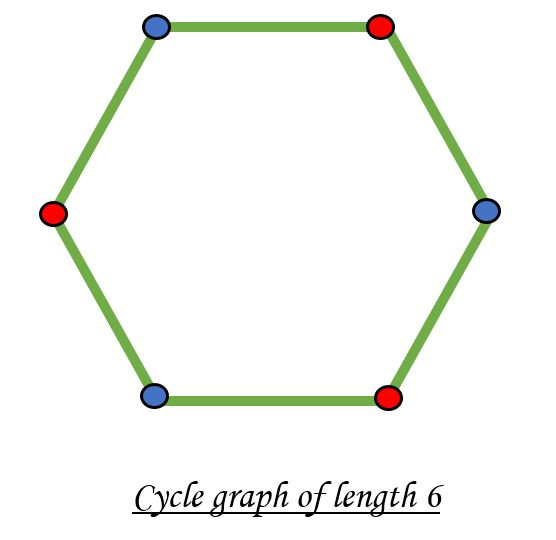
\includegraphics[scale=0.5]{../material/images/bipartite-graph-six-nodes.jpg}
    \caption{bipartiter Graph mit Kreis der Länge sechs \parencite{GeeksforGeeks2018}}
    \label{fig:bipartite-six-nodes}
\end{figure}

\begin{figure}
    \centering
    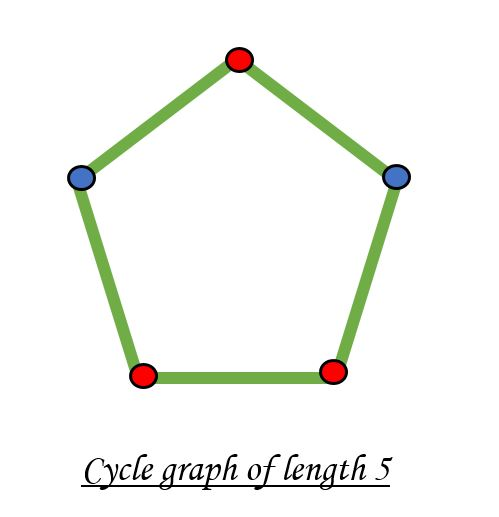
\includegraphics[scale=0.5]{../material/images/bipartite-graph-five-nodes.jpg}
    \caption{nicht bipartiter Graph mit Kreis der Länge fünf \parencite{GeeksforGeeks2018}}
    \label{fig:bipartite-five-nodes}
\end{figure}

Wie läuft das Beispiel nun konkret ab. Zunächst werden die Daten eingelesen. Dies
erfolgt zur Vereinfachung über eine Datei. Dies kann jedoch jederzeit auf eine
alternative Eingabe umgestellt werden, zum Beispiel um die Daten von einem
Messaging-System wie Apache Kafka einlesen zu können. Dabei ist zu beachten,
dass die Bibliotheken unterschiedliche Eingabeformate unterstützen. Anschließend
werden die Daten an eine beliebige Ausgabe gesendet. Dies ist in unserem Fall die
Konsole. Wie auch schon die Eingabe kann hier natürlich auch eine andere Möglichkeit
genutzt werden.

\subsection{Architektur der Referenz-Implementierung}
Jede Streaming-Anwendung von Apache Flink wird als Job bezeichnet. Diese
Bezeichnung wird oft im Batch-Bereich benutzt. Eine Streaming-Anwendung besteht
aus zwei Teilen der Initialisierung der Streaming-Umgebung und der eigentlichen
Anwendung, welche dem EVA-Prinzip folgt. Zunächst muss die Streaming-Engine
initialisiert werden. Dabei ist es von Vorteil zu wissen, ob die spätere Anwendung
nur lokal oder remote betrieben werden soll. Lokal bedeutet in diesem Zusammenhang,
dass die Anwendung einen Apache Flink Cluster in der selbem \gls{JVM} startet.
Dies lässt sich bereits bei der Entwicklung fest einprogrammieren oder dynamisch
von Apache Flink bestimmen lassen. Die Streaming-Umgebung ist ein sehr wichtiges
Management-Objekt, welches für verschiedene Aufgaben vom Entwickler benutzt
werden sollte.

\foreigntextquote{english}[\cite{Foundation2018}]{
The LocalStreamEnvironment is a StreamExecutionEnvironment that runs the program
locally, multi-threaded, in the JVM where the environment is instantiated. It
spawns an embedded Flink cluster in the background and executes the program on
that cluster.}

Danach können die eigentlichen Daten eingelesen werden. Dazu kann ein von Apache
vordefinierter Connector zum Beispiel für Dateien benutzt werden oder eine
Bibliothek. In diesem Beispiel wird der File-Connector benutzt, welcher im Kern
von Apache Flink enthalten ist. Dieser kann einfach über die Streaming-Umgebung
aufgerufen werden. Wenn andere Connectoren zum Einsatz kommen sollen, werden
diese initialisiert und anschließend bei der Streaming-Umgebung registriert.

Die Umwandlung von Text zu Kanten muss für jede Anwendung neu definiert und
programmiert werden. Im Beispiel liegen die Daten wie schon erwähnt in einer
Datei vor. Dabei besteht jede Zeile aus genau einer Kante. Jede Kante besteht
dabei aus zwei Identifikationsnummern für die Kanten, welche durch einen
Tabulator getrennt sind. Alle Kanten sind in Apache Flink gerichtete Kanten.
Eine ungerichtete Kante kann nur erzeugt werden, wenn es eine zweite Kante gibt,
bei der die Anfangs- und End-Identifikationsnummern vertauscht sind.

\foreigntextquote{english}[\cite{Foundation2018}]{
In Gelly an Edge is always directed from the source vertex to the target vertex.
A Graph may be undirected if for every Edge it contains a matching Edge from the
target vertex to the source vertex.}

Anschließend erfolgt die Datenverarbeitung. Dabei wird auch die Ausgabe mit
definiert. Im Beispiel wird der Graph getestet, ob dieser bipartite ist. Dabei
werden die Daten in einem temporären Stream mit Fenster zwischengespeichert. Die
Überprüfung wird in eine Aggregationsfunktion eingebettet, um die
Zwischenergebnisse zu speichern. Als letztes wird der Job dann gestartet. Dabei
wird in der lokalen Umgebung dann der Cluster gestartet.

\subsection{Entwurf von \enquote{graphstream-project}}
Die Umsetzung des Beispieles ist ähnlich wie eine normale Java-Anwendung zu
programmieren. Zunächst wird die Eingabe definiert. In \enquote{graphstream-project}
werden Eingabe-Komponenten als \enquote{Sources} bezeichnet. Hier in diesem
Beispiel werden die Graph-Daten wieder von einer Datei bereitgestellt. Die
Bibliothek stellt ein Protokoll zur Datenübertragung bereit. Dadurch ist eine
einfache Kommunikation auch mit anderen Systemen möglich. Das Protokoll hat dabei
Ähnlichkeiten zum \enquote{Portable Bitmap File} Format. Beide Protokolle haben
am Anfang einen Kopf für die Meta-Informationen bevor die eigentlichen Daten
folgen. Im Unterschied zu \enquote{gelly-streaming} lassen sich die Kanten
genau spezifizieren.

\foreigntextquote{english}[\cite{Team2018}]{
ae Allows to add an edge. This command must be followed by the unique identifier
of the edge, and then the identifiers of two other nodes. As for nodes, you can
specify a parameter list. It is possible to create directed edges by adding a
“>” (greater-than) or “<” (smaller-than) character between the nodes identifiers.
This indicates the direction of the edge. When no “<” or “>” is present, the
edge is not directed.}

Die Quelle wird dann mit einer Graph-Instanz verbunden. Denn es ist möglich
den Graphen durch den Aufruf von Methoden zu ändern.

Die Implementierung von Algorithmen erfolgt bei \enquote{graphstream-project}
über das Interface Algorithm. Dieses stellt zwei Methoden bereit init und compute.
Die Methode init bekommt einen Graphen übergeben und initialisiert den Algorithmus.
Anschließend erfolgt die Manipulation des Graphen in der compute Methode.
Abschließend werden die Resultate des Algorithmus über selbst programmiert
Getter bereitgestellt. Die Ausgabe erfolgt über einen Aufruf der Konsole.

\subsection{Entwurf von \enquote{Gephi}}
Die Umsetzung des Beispieles von Gephi ist anders, als die anderen. Dort
existieren mehrere Möglichkeiten, die Aufgabenstellung zu lösen.

Die erste Möglichkeit besteht darin ein neues Statistik-Plug-In zu entwickeln
und das bestehende Streaming-Plug-In nur für die Datenübertragung zu verwenden.
Dies hätte den Vorteil, dass sehr viel von \enquote{Gephi} übernommen werden
kann und nicht in die Kommunikation eingegriffen werden muss. Der Graph muss
dabei von einem externen Service bereitgestellt werden und über HTTP übertragen.
Ob der Service die Daten selbst erzeugt oder diese zum Beispiel von einem
externen Anbieter wie Apache Kafka ausließt, hängt von den Anforderungen ab. Der
Service muss lediglich in der Lage sein, die Daten entsprechend transformieren
zu können. Die Berechnung würde dann im Programm erfolgen ebenso die Ausgabe.

Die andere Möglichkeit ergibt sich durch die direkte Benutzung des
Streaming-Plug-Ins. Das Streaming-Plugin von \enquote{Gephi} basiert wie schon
beschrieben auf HTTP. Dabei kann \enquote{Gephi} beide Seiten der
Client-Server-Verbindung repräsentieren je nach Anwendungsfall. Die
Datenübertragung erfolgt dabei standardmäßig im JSON-Format. Wenn \enquote{Gephi}
als Client betrieben wird, meldet es sich bei einem externen Service an und wartet
anschließend bis vom Service Daten gesendet werden, um diese anzuzeigen. Im
Serverbetrieb läuft \enquote{Gephi} mit einem Arbeitsbereich als Master. Dies
bedeutet, dass sich externe Services und andere \enquote{Gephi} Anwendungen am
Master anmelden können. Werden anschließend die Daten am Master durch den
Benutzer verändert oder ein Teilnehmer verändert seine eigenen Daten, dann wird
diese Information über den Master an alle Teilnehmer weitergeleitet.

Durch die beiden Seiten ergeben sich zwei mögliche Varianten bei der Benutzung
des Streaming-Plug-Ins. Die erste Variante ist es, die vorhandene \gls{API}
anzupassen. Um nicht nur den Graphen zu manipulieren, sondern auch um Statistiken
über den Graphen abfragen zu können. Die andere Variante besteht darin, einen
speziellen Event-Handler zu schreiben, der eine spezielle Funktion beim Eingang
von Ereignissen umsetzt. Da beim Eingang von Ereignissen im Standardfall nur der
Graph aktualisiert wird. Um die gewünschte Funktion umzusetzen, muss ein extra
Plug-In geschrieben werden, da einige Komponenten von der \gls{API} benötigt
werden. Das Listing \ref{code:GephiGraphHandler} zeigt den prototypischen Einsatz
eines solchen Handlers. Dieser Handler kann dann alle gewünschten Operationen
ausführen je nach Anwendungsfall. Diese Variante ist jedoch Abstraktionsebene
tiefer als, wenn der StreamingController direkt verwendet wird. Der
StreamingController erlaubt es jedoch nur Event-Handler zu registrieren, welche
auf Ereignisse reagieren können, wenn der Stream geschlossen wird.

\begin{listing}
    \inputminted[breaklines=true]{java}{../material/code/GephiGraphHandler.java}
    \caption{prototypischer Einsatz für einen GraphHandler}
    \label{code:GephiGraphHandler}
\end{listing}

\section{Vergleich der Designs und Beschreibung der Probleme}
Eine Vergleich der verschiedenen Bibliotheken und der jeweiligen Designs ist
schwierig, da die Bibliotheken über unterschiedlichste Entwicklungsstände
verfügen und auch verschiedenen Ansätze verfolgen, wie schon in den Grundlagen
erläutert wurde.

Zunächst benutzen die Bibliotheken unterschiedliche Informationen und Darstellungen
für die Graph-Daten. Die Referenz \enquote{gelly-streaming} stellt dabei die
wenigsten Informationen bereit. Dies liegt natürlich an den verschiedenen
Konzepten der Bibliotheken. Es existieren zwei Arten von Informationen, die
eigentlichen Graph-Daten und Meta-Informationen, welche zusätzliche Informationen
zu den Graph-Daten bereitstellen. Bei \enquote{gelly-streaming} gibt es keine
Meta-Informationen und es werden lediglich die Kanten als Graph-Daten verarbeitet.
Eine Kante besteht dabei aus zwei IDs und einem Wert. Sowohl der Wert als auch
die IDs können dabei beliebige Datentypen annehmen. Es gibt lediglich eine
Einschränkung, dass beide IDs den selben Typ angehören müssen. Die Knoten werden
aus den IDs der Kanten erzeugt und haben sonst keine zusätzlichen Werte. Die
beiden anderen Bibliotheken stellen umfangreichere Daten bereit. Dort existieren
sowohl Meta-Informationen, als auch die bei \enquote{gelly-streaming} fehlenden
Knoten. Ob diese Informationen letzlich immer benötigt werden hängt natürlich
von den Anforderungen der jeweiligen Anwendung ab. Ein Entwickler könnte die
zusätzlichen Meta-Informationen mit übermitteln. Dies hat jedoch zur Folge, dass
der einzelne Wert dann immer ein komplexer Datentyp sein muss, wie zum Beispiel
eine Map, Liste,~\dots oder eine eigene Klasse.

In diesem Zusammenhang ist noch wichtig zu erwähnen, dass \enquote{gelly-streaming}
keinen weiteren Zugriff auf die Knoten, bis auf die IDs, hat im Gegensatz zu \enquote{gelly}.
Da nur Kanten eingelesen werden und Knoten automatisch aus den Ids der Kanten
erzeugt werden. Ein Entwickler ist also immer gezwungen, sich die Daten der
Knoten bei Bedarf nachzuladen. Dieses Phänomen ist auch als lazy-loading bekannt
und kommt bei Anwendungen mit Datenbanken zum Tragen.

Wie schon oben erwähnt, könnte ein Entwickler die zusätzlichen Daten mit
übertragen und dann bei \enquote{gelly-streaming} die Konvertierung übernehmen.
Allerdings wird dann das nicht vorhandene Protokoll von \enquote{gelly-streaming}
zum Problem. Der Entwickler hat zwar die Freiheit beliebige Daten zu übertragen,
allerdings muss bei jedem neuen Projekt genau definiert werden, wie die zu
übertragenden Daten auszusehen haben. Dies kann gerade bei vielen Projekten zum
Problem werden. Da im Standartfall einfach eine Zeichenkette zur Verfügung steht.
Es existieren allerdings schon Ansätze diese Problematik zu lösen. Apache Flink
stellt Basisklassen für verschiedene Dateiformate bereit zum Beispiel
BinaryInputFormat, CsvInputFormat,~\dots . Damit kann ein Entwickler konkrete
Protokolle definieren bzw. gibt bei einer CSV-Datei nur die Trennzeichen an.

Die Referenz \enquote{gelly-streaming} hat Vorteile, bei der Streaming-Umgebung
und der Verteilung. Dies kommt natürlich daher, dass Apache Flink in diesen
Punkten schon über einen guten Entwicklungsstand verfügt. Darum ist
\enquote{gelly-streaming} auch die einzige Bibliothek, welche sich verteilt
betreiben lässt. Beim Vergleich der gesamten Streaming-Umgebung ist
\enquote{gelly-streaming} klar am fortschrittlichsten. Es gibt ein eigenes
Konzept für Streams, welches je nach Anforderung konfiguriert werden kann. In
unserem Beispiel soll ein einfacher Test nach Ablauf eines Zeitfensters
durchgeführt werden. Bei \enquote{gelly-streaming} wird zur Lösung dieses
Problems eine Window-Stream über den Test konfiguriert. Bei \enquote{graphstream-project}
wird ein anderer Event-System-Ansatz gewählt. Dort hat der Entwickler die
Möglichkeit zu entscheiden, ob alle Events auf einmal eingelesen werden sollen
oder nicht. Die Möglichkeit konkrete Zeitfenster zu definieren gibt es bei
\enquote{graphstream-project} nicht. Es kann lediglich abgefragt werden, ob noch
neue Events vorhanden sind. Auf die eigentlichen Events kann jedoch nicht
zugegriffen werden, sondern lediglich auf den vollständigen Graphen. Das Listing
\ref{code:GraphStreamInput} zeigt den Ablauf zum Einlesen von Events. Bei \enquote{Gephi}
kann über einen speziellen GraphEventHandler auf die Events zugegriffen werden.
Allerdings ist auch dort kein Zeitfenster vorgesehen.

\begin{listing}
    \inputminted[breaklines=true]{java}{../material/code/GraphStreamInput.java}
    \caption{prototypischer Ablauf zum Einlesen von Daten bei \enquote{graphstream-project}}
    \label{code:GraphStreamInput}
\end{listing}

Beim Vergleich der Unterstützung von Algorithmen haben alle Bibliotheken noch
große Problem, obwohl bei \enquote{gelly-streaming} eigentlich mehr zu erwarten
wäre aufgrund der Verbindung zu Apache Flink und der Bibliothek \enquote{Gelly}.
Denn dort werden schon einige Graph-Algorithmen definiert, welche jedoch nicht in
\enquote{gelly-streaming} verwendet werden. Des Weiteren stellt \enquote{Gelly}
ein Interface GraphAlgorithm bereit, womit ein Entwickler eigene Graph-Algorithmen
entwickeln kann. Diese Möglichkeit gibt es bei \enquote{gelly-streaming} nicht.
Dies hat dort auch zur Folge, dass alle selbst definierten Algorithmen eine
Erweiterung vom SummaryAggregation sein müssen. Dies macht eine Entwicklung
neuer Algorithmen schwerer. Denn die Algorithmen bei \enquote{Gelly} werden als
Map-Reduce-Probleme beschrieben. Beim Interface GraphAlgorithm ist dies so vorgesehen,
denn dieses Interface hat nur eine run-Methode in der die konkreten
Methodenaufrufe gekapselt werden. Bei \enquote{graphstream-project} existiert
ebenfals ein Interface Algorithm für die Implementierung von Graph-Algorithmen.
Dies ist als sogenanntes Marker-Interface konzipiert. Das bedeutet, dass alle
Klassen, welche dieses Interface implementieren einen Graph-Algorithmus darstellen.
Jedoch wird dieses Interface nicht in anderen Klassen für zum Beispiel
Polymorphismus,~\dots~eingesetzt. Dies lässt sich auch ganz klar an der
Interface-Struktur ablesen. Das Interface selbst besteht aus zwei Methoden.
Die init-Methode ist für die Initialisierung des Algorithmus zuständig und die
compute-Methode für die Berechnung. Die Rückgabewerte müssen über selbst
definierte Getter an den Aufrufer zurückgegeben werden. Um das Interface für
Polymorphismus nutzten zu können, müsste jedoch eine Möglichkeit für die
Rückgabewerte existieren. Dies ist aber im Interface nicht vorgesehen. Um diese
Einschränkung aufzuheben, muss entweder das Interface angepasst werden um eine
Getter Methode oder die compute-Methode wird um einen Rückgabewert erweitert.
Allerdings ergibt sich dabei die Frage, was passiert, wenn mehr als ein
Rückgabewert benötigt wird.

Nachdem die Designs analysiert wurden, wird nun deren praktische Umsetzung
beschrieben und welche Problem dabei auftraten.

\chapter{Realisierung}
In diesem Kapitel geht es darum, die wichtigsten Punkte der Realisierungen
zu beschreiben. Die Bibliothek \enquote{gelly-streaming} wird dabei wieder als
Referenz benutzt. Anschließend werden die Realisierung und deren Benutzbarkeit
analysiert und mögliche Lösungsen beschrieben.

\section{Analyse der Umsetzung}
Die Umsetzung der jeweiligen Versionen erfolgte nach den Methoden der
Softwareentwicklung. Dabei wurden die Entwürfe aus dem vorangegangen Kapitel
als Grundlage benutzt. Zusätzlich wurden die jeweiligen Dokumentationen und
Beispiele der Bibliotheken als Basis benutzt. Die verwendeten Testfälle wurden
dabei für die jeweilige Bibliothek angepasst. Des Weiteren lassen sich daraus
schnell und einfach weitere Testfälle erzeugen.

\subsection{Umsetzung der Referenz-Implementierung}
Die Referenz-Implementierung basiert auf dem Beispiel aus der Bibliothek. Der
wesentliche Unterschied zur Umsetzung aus der Bibliothek ist, dass die
Bibliothek Picocli\footnote{\url{https://picocli.info/}} für die Kommandozeile
benutzt wurde. Dies sorgt dafür, dass die Anwendung sich gut erweitern lässt.
Das Listing \ref{code:BipartiteGellyStreaming} zeigt den Code wie es in der
Bibliothek umgesetzt ist. Bei der Analyse des Beispieles fällt auf, dass die
Anwendung vier Informationen benötigt:

\begin{itemize}
\item dem Pfad für die Kanten
\item dem Pfad für die Ausgabe
\item dem Zeitinterwall für das Fenster
\item dem Trennzeichen für die Kanten
\end{itemize} 

\begin{listing}
\inputminted[breaklines=true]{java}{../material/code/BipartitenessCheckExample.java}
\caption{Umsetzung von Bipartitness von \enquote{gelly-streaming} \cite{Kalavri2018}}
\label{code:BipartiteGellyStreaming}
\end{listing}

Die ersten beiden Parameter sind dabei die wichtigsten. Die beiden anderen
Parameter sind im Beispiel schon definiert. Das Zeitintervall hat dabei eine
Länge von 500ms und das Trennzeichen ist das Tabzeichen. In der Methode
\enquote{parseParameters} werden die Paramter der Kommandozeile analysiert und
ggf. ein starten der Anwendung verhindert. Es sind dabei nur zwei Zustände
erlaubt. Der erste Zustand ist, wenn gar keine Parameter übergeben werden. Dann
werden die Kanten automatisch erzeugt und die Ergebnisse auf der Konsole
ausgegeben. Der zweite Zustand ist, wenn beide Parameter übergeben werden. Dann
werden die Kanten aus der Datei gelesen und auch in eine Datei geschrieben. Ein
Blick in die main-Methode zeigt jedoch, dass sich auch die Ausgabe über eine
Variable steuern lässt. Dies wird jedoch nicht genutzt. Der Grund dafür liegt
klar in der schlechten Transformation der Kommandozeilenparameter. Falls die
Anwendung dahingehend verändert wird, dass jemand nur einen einzigen Parameter
übergeben muss und jemand dies auch tut, kann die Anwendung nicht unterscheiden,
ob es sich dabei um den Pfad für die Kanten oder um dem Ausgabepfad handelt.

Das Problem des Beispiel ist, dass hier zwei verschiedene Konzepte falsch
verwendert werden. Nämlich die Konzepte von Optionen und Argumente wie, sie in
jeder Kommandozeile zum Einsatz kommen, wie zum Beispiel bei Linux dort sind die
meisten Programme Kommandozeilenanwendungen. Argumente sind Variablen, welche für
die Erfüllung der Aufgabe notwendig sind. Im Gegensatz dazu sind Optionen
Schalter, welche es dem Benutzer ermöglichen, gewisse Basiswerte zu verändern.
Ein klassisches Beispiel ist ein SSH- oder FTP-Client, diese ermöglichen es den
jeweiligen Port über eine Option zu ändern, dies ändert jedoch nicht die
Anwendungslogik. Wenn ein Benutzer jedoch keine Address mitgibt, dann wird der
Client eine Fehlermeldung ausgeben, denn die Address ist hier ein Argument. In
dem Beispiel müssten deshalb sowohl der Dateipfad für die Kanten als auch der
Dateipfad für die Ausgabe Optionen sein, denn es spielt für die Anwendung ja
keine Rolle ob die Pfade übergeben werden oder nicht. Denn wenn kein Dateipfad
für die Kanten übergeben werden, werden die Kanten generiert und wenn kein
Ausgabepfad übergeben wird, dann werden die Daten einfach in die Konsole
ausgegeben.

In der veränderten Realisierung wird dies auch so umgesetzt. Das Listing \ref{code:BipartiteReferenz}
zeigt den veränderten Code. Dabei wir der Fall entfernt, dass kein Dateipfad
für die Eingabedatei übergeben wurde. Der Dateipfad für die Kanten ist jetzt ein
verplichtendes Argument der Anwendung. Alle weiteren Daten wie Ausgabepfad,
Zeitintervall und Trennzeichen sind jetzt Optionen und können bei Bedarf angepasst
werden. Dadurch ist es schnell möglich die Eingabedatei zu ändern oder das
Zeitintervall anzupassen. Alle möglichen Argumente und Optionen werden dabei als
private Variablen angelegt und mit Annotationen versehen. Diese werden anschließend
von der Bibliothek verarbeitet.  Ein Problem bei der Implementierung bleibt aber
bestehen, in der \enquote{getEdgesDataSet} werden die Daten von der Umgebung
gelesen und gleichzeitig in Objekte transformiert. Für eine optimale Umsetzung
müsste das Einlesen der Daten getrennt von der Transformation erfolgen.
Dies spielt genau dann eine Rolle, wenn die Eingabequelle nicht mehr eine Datei,
sondern zum Beispiel ein Messaging-System ist. Da die Transformation der
Daten trotzdem erfolgen muss, egal welche Eingabequelle vorhanden ist und ein
Entwickler dann nicht mehr die \enquote{readTextFile}-Methode aufrufen kann.

\begin{listing}
\inputminted[breaklines=true]{java}{../material/code/GellyStreamingResult.java}
\caption{Umsetzung von Bipartitness für \enquote{gelly-streaming}}
\label{code:BipartiteReferenz}
\end{listing}

Die Ausgabe für verschiedene Eingaben hat Ähnlichkeiten zu einem
\gls{JSON}-Dokument. Allerdings erschließt sich dem Betrachter die genaue
Struktur des Formates nicht. Das Listing \ref{code:BipartiteGellyResult} zeigt
exemplarisch die Ausgabe von einem bipartiten Graphen.

\begin{listing}
\begin{minted}{text}
(true, {1= {
        1=(1,true),
        2=(2,false),
        3=(3,true),
        4=(4,false),
        5=(5,true),
        6=(6,false)}
})
\end{minted}
\caption{Ausgabe \enquote{gelly-streaming} für bipartiten Graph}
\label{code:BipartiteGellyResult}
\end{listing}

Des Weiteren ergeben sich Probleme bei der Verwendung der Streaming-Umgebung.
Apache Flink kennt wie schon erwähnt zwei mögliche Laufzeitumgebungen den lokalen
Cluster und einen eigenen Cluster. Diese beiden Umgebungen sorgen jedoch bei
der Erstellung und der Ausführung des Archives für Probleme. Falls ein externer
Cluster benutzt wird, braucht das Archive nicht die Klassen des Clusters
enthalten. Im Gegensatz dazu braucht der lokale Cluster die Klassen. Dies macht
jedoch eine Entwicklung per \gls{IDE} schwierig. Da diese nicht unterscheiden
kann, wann die zusätzlichen Bibliotheken benötigt werden und wann nicht. Um
dieses Problem zu lösen, werden entweder Maven-Profile benötigt oder es werden
die Klassen einfach immer mit in das Archive gepackt. Allerdings hat dieses auch
zwei Nachteile. Der erste Nachteil ist, dass sich der Speicher des Archives
erhöht. Dieser Punkt ist nicht so entscheident. Der zweite Nachteil ist dagegen
nicht zu verachten. Falls alle Klassen im Archive sind und die Anwendung auf
einem externen Cluster gestartet wird, der ebenfalls die Klassen beinhaltet,
dann werden Klassen überschrieben. In der Regel werden dies die Klassen des
Clusters sein. Dies kann jedoch dazuführen, dass verschiedene Versionen
Inkompatibilitäten hervorrufen.

\subsection{Umsetzung von \enquote{graphstream-project}}
Für die erfolgreiche Umsetzung waren zwei Schritte notewendig. Als erstes wurde
der Algorithmus implementiert. Dazu wurde eine Klasse erstellt, welches das
Algorithm-Interface implementiert, wie es alle Algorithmen von
\enquote{graphstream-project} machen. Anschließend wurde die Hauptklasse
geschrieben, welche die Daten einliest und den Algorithmus auffruft.
Das Listing \ref{code:GraphStreamProjectResult} zeigt die Hauptklasse mit dem
Ablauf zum einlesen der Daten. Die Besonderheit bei dieser Lösung ist, dass
der Graph bei der Quelle registriert wird und dadurch über ein Event-System
automatisch aktualisiert wird. Eine Konvertierung der Eingabedaten ist nicht
erforderlich, da \enquote{graphstream-project} ein Protokoll bereitstellt und
die Transformation automatisch beim Einlesen der Daten übernimmt.

\begin{listing}
\inputminted[breaklines=true]{java}{../material/code/GraphStreamProjectResult.java}
\caption{Umsetzung von Bipartitness für \enquote{graphstream-project}}
\label{code:GraphStreamProjectResult}
\end{listing}

Wie schon im Entwurf beschrieben ist es nicht möglich die Events abzufragen,
sondern lediglich ob noch weitere Events vorhanden sind. Ebenso ist es nicht
möglich ein Zeitfenster festzulegen, wie dies bei \enquote{gelly-streaming}
der Fall ist. Eine Möglichkeit für ein Zeitfenster ist es, wenn am Ende der
Verarbeitung die \gls{JVM} den gewünschten Zeitraum wartet. Dies müsste
allerdings genauer getestet werden, ob sich dadurch nicht irgendwelche anderen
Problemfälle ergeben.

Wie bei \enquote{gelly-streaming} ist es bei \enquote{graphstream-project}
möglich mehrere Algorithmen hintereinander auszuführen. Allerdings gibt es einen
wichtigen Unterschied zwischen beiden Bibliotheken. Bei \enquote{graphstream-project}
liegt der Graph direkt als Objekt vor. Dadurch ist der Entwickler jedoch in
der Lage den Graphen über einen Algorithmus zu manipulieren und dadurch denn
Ablauf zu verfälschen. Bei \enquote{gelly-streaming} ist dies nicht der Fall.
Dort ist der Ablauf wie bei einer Filterkette. Die eingehenden Daten werden
verarbeitet und an die nächste Einheit weitergereicht, usw. bis zur letzten
Einheit. Wenn anschließend neue Daten ankommen, laufen diese durch den selben
Prozess ohne von den alten Daten beeinflusst zu werden.

Bei der Ausgabe ist \enquote{graphstream-project} besser als
\enquote{gelly-streaming}. Denn bei \enquote{graphstream-project} kann der
Entwickler die Ausgabe komplett selbst definieren oder diese auch komplett
weglassen. Das Listing \ref{code:BipartiteGraphStreamResult} zeigt die Ausgabe
eines bipartiten Graphen. Jede Zeile steht dabei für ein ankommendes Event. In
unserem Beispiel enthalten die Beispieldaten Events zur Erzeugung von Kanten und
Knoten. Da die Knoten nicht automatisch mit erzeugt werden, jedoch Vorraussetzung
für die Erstellung der Kanten sind.

\begin{listing}
\begin{minted}{text}
The graph is bipartite: true
The graph is bipartite: true
The graph is bipartite: true
The graph is bipartite: true
The graph is bipartite: true
The graph is bipartite: true
The graph is bipartite: true
The graph is bipartite: true
The graph is bipartite: true
The graph is bipartite: true
The graph is bipartite: true
The graph is bipartite: true
The graph is bipartite: true
The graph is bipartite: true
The graph is bipartite: true
\end{minted}
\caption{Ausgabe \enquote{graphstream-project} für bipartiten Graphen}
\label{code:BipartiteGraphStreamResult}
\end{listing}

\subsection{Umsetzung von \enquote{Gephi}}
Im Gegensatz zu den beiden anderen Implementierungen konnte \enquote{Gephi}
nicht erfolgreich umgesetzt werden, obwohl die Entwürfe mit fortgeschrittenen
Java-Kentnissen umsetzbar sein müssten. Aufgrund der Architektur und dem
technischen Fortschritt liesen sich die Entwürfe nicht umsetzten.

Die Anwendung \enquote{Gephi} ist wie schon erwähnt eine Netbeans-Anwendung.
Dabei besteht die Anwendung aus einem Kern und zusätzlichen Plug-Ins, welche den
Kern um weitere Funtionalität ergänzen. Daran ist auf den ersten Blick auch
nichts ausszusetzten, denn andere Anwendungen wie Eclipse,
Jetbrains IntelliJ IDEA arbeiten,~\dots arbeiten nach dem selben Prinzip.
Allerdings bergen solche Architekturen immer auch Risikos. Zum einen besteht die
Gefahr, dass falls ein Benutzer zu viele Plug-Ins aktiviert, diese sich
gegenseitig behindern oder sogar das Programm zum Absturz bringen
können. Ein anderes Problem sind zu viele und unklare Abhängigkeiten auch als
\enquote{Dependency-Hell} bekannt. Dabei werden zwischen einzelnen
Komponenten Abhängigkeiten geschaffen, welche wiederum Abhängkeiten zu anderen
Komponenten haben und somit ein komplexes Netzwerk von Abhängigkeiten entsteht,
welches der Entwickler weder durchschauen, noch dieses mit relativ überschaubaren
Aufwand auflösen kann.

Der Kern von \enquote{Gephi} besteht aus circa 70 Modulen. Bei einem genaueren
Blick auf die einzelnen Module stellt der Betrachter fest, dass es Module gibt,
welche keine Funktionalität bereitstellen, wie zum Beispiel bei dem Modul
\enquote{CoreLibraryWrapper}. Diese Module dienen lediglich dazu verschiedene
Abhängigkeiten zu bündeln. Dieser Vorgang wird durchgeführt um möglichst ähnliche
Komponenten, welche in vielen Modulen zum Einsatz kommen sollen für den Entwickler
leichter verfügbar zu machen. Bei dem Modul \enquote{CoreLibraryWrapper} ist
dies jedoch nicht der Fall. Diese Modul bündelt zwar andere Abhängkeiten und wird
selber von vielen Modulen als Abhängkeit benutzt, jedoch sind die gebündelten
Abhängigkeiten sehr verschieden. Denn dort sind Hilfsbibliotheken wie
\enquote{Apache Commons Codec} und Bibliotheken zur Darstellung wie
\enquote{JFreeChart} enthalten. Dies sorgt jedoch für Probleme, denn nicht alle
Module benutzen auch alle bzw. viele von diesen Abhängkeiten, sondern die meisten
nutzen nur einige wenige. Dadurch ist ein Entwickler gezwungen sich alle Module
anzusehen, falls er in seinem Modul einen Fehler entdeckt hat und diesen nur
durch eine andere Version einer Bibliothek aus \enquote{CoreLibraryWrapper} zu
lösen ist.

Dieses Abhängigkeitsproblem allein ist für sich genommen erstmal noch kein
Problem. In Kombination mit einem zweiten Problem bricht das ganze System jedoch
zusammen. Das zweite Problem ist die Entwicklung der Programmiersprache Java,
welche \enquote{Gephi} nicht ständig kontrolliert hat und dadurch seine eigenen
Entwicklung behindert hat. Ob die Entwicklung von Java die Entwicklung von
\enquote{Gephi} beeinflusst hat oder ob die Entwicklung von \enquote{Gephi}
stagnierte und anschließend nur schwer wieder aufgenommen werden konnte lässt
sich nicht mit Sicherheit festellen. Wie bei vielen neuen Entwicklungen, war es
auch bei Java so, dass diese über einige Kinderkrankheiten verfügte. Diese haben
die Entwickler anschließend in eigenen Bibliotheken gelöst und der Allgemeinheit
zur Verfügung gestellt. Dies wurde gerade zur Anfangszeit von Java durchgeführt.
In unserem Fall trifft dies auf eine StAX-Bibliothek zur Verarbeitung von
\gls{XML}-Dateien zu. Diese Bibliothek wurde in Java 6 Standard. Davor musste ein
Entwickler diese Funktionen über eine Bibliothek bereitstellen. 

\textquote[\cite{Ullenboom2019}]{
Die Pull-API StAX inklusive Implementierung ist Teil der Standardbibliothek und
JDK/JRE ab Version 6. [Um die API vor Java 6 nutzen zu können, kann unter 
\url{http://stax.codehaus.org/} eine Implementierung der API bezogen werden. ]
Mit ihr lassen sich XML-Dokumente sehr performant ablaufen, jedoch nicht ändern.
}

Die StAX-Bibliothek wird seit 2007 nicht mehr aktiv weiterentwickelt, denn im
Jahr 2006 wurde Java 6 veröffentlicht und wurde dadurch nicht mehr benötigt.
Daraus folgt die Entwickler hatten mehr als ein Jahr Zeit ihren Codebasis
anzupassen. In der Realität war sogar mehr als ein Jahr Zeit, denn die
Bibliotheken werden ja normalerweise nicht gelöscht. Jedoch hat Sun bzw. Oracle
den Support für Java 5 im Jahr 2009 bzw. für Java 6 im Jahr 2013 eingestellt.
Dadurch wurde die StAX-Bibliothek ebenfalls nicht mehr benötigt und wurde
entfernt. 

Beide Problem zusammen sorgen für die nur noch marginale Weiterentwicklung bzw.
Benutzbarkeit von \enquote{Gephi}. Denn viele Module haben eine Abhängkeit zu
\enquote{CoreLibraryWrapper} benutzen jedoch nicht alle dadurch bereitgestellten
Bibliothek. Dadurch ist es nicht einfach möglich die Abhängkeit von StAX zu löschen,
da es bei den vielen Modulen nicht klar offensichtlicht ist, ob die Module StAX
benutzen oder nicht. Um dieses Problem insgesammt lösen zu können muss das Modul
\enquote{CoreLibraryWrapper} komplett entfernt werden. Im zuge der Entfernung
müssen alle Module, welche die StAX-Bibliothek verwenden auf Java 6 oder moderner
portiert werden. Allerdings dürfen die Module auch nicht auf eine der aktuellsten
Versionen wie Java 9 oder später portiert werden, denn dort wurden Bibliothek
welche sowohl extern als auch im JDK enthalten waren entfernt. Zu diesen Bibliothek
gehörten zum Beispiel Bibliothek für die \gls{XML}-Verarbeitung. Dieser Vorgang
wurde durchgeführt um einerseits den JDK zu verschlanken und andererseits um
JavaSE von JavaEE bzw. JakartaEE sauber zu trennen.

\section{Bewertung der Umsetzungen}
Ein Vergleich der verschiedenen Umsetzungen ist nicht leicht, da einerseits die
Bibliotheken sehr unterschiedliche Ansätze benutzen und andereseits die
Implementierung mit \enquote{Gephi} nicht umsetzbar war. Dies heißt nicht
automatisch, dass die Bibliothek \enquote{Gephi} schlecht ist. Sie ist lediglich
im Moment nicht benutzbar, lässt sich jedoch wie oben beschrieben auch beheben.
Wenn jemand \enquote{Gephi} verbessert, kann es durchaus sinnvoll sein sich die
gesammte Architektur bzw. die Infrastruktur anzusehen und ggf. diese vorher
anzupassen. Wenn sich durch diese Betrachtung jedoch ergibt, dass die gewählte
Technologie mit Netbeans nicht geeignet ist, ist ein Blick auf die
funktionierenden Bibliotheken anzuraten. Je nachdem wie viele Resourcen zur
Verfügung stehen. Denn, dass der Ansatz über Plug-Ins funktioniert zeigen ja,
gerade Beispiele, wie Eclipse, IntelliJ IDEA,~\dots . Der Netbeans \gls{IDE}
unterstützt dies natürlich auch.

Wenn nur die beiden funktionierenden Umsetzungen betrachtet werden, wird einem
klar, dass beide Bibliothek im begrenzten Umfang Graph Streaming durchführen.
Denn einerseits können die Bibliotheken Daten von einer unbegrenzten Liste
einlesen, zum Beispiel von Apache Kafka, was ja die Definition eines Streams
ausmacht. Zum anderen handelt es sich bei den Daten ja um Kanten also um
Graph-Daten, welche verarbeitet werden.

Beim einlesen der Daten sind beide Bibliotheken gleich gut, da beide
verschiedensten Connectoren bereitstellen bzw. dem Entwickler die Möglichkeit
geben eigene zu entwickeln. Was die eigentlichen Daten angeht haben beide, wie
schon erwähnt ähnliche Möglichkeiten. Deshalb wird es, was die Daten angeht sehr
stark auf den jeweiligen Anwendungsfall ankommen. Wenn für die gewünschte Analyse
lediglich die Kanten mit ihren Werten benötigt werden bzw. die Knoten nur sehr
selten, dann ist die Verwendung von \enquote{gelly-streaming} ausreichend. Zum
Beispiel bei klassischen statischen Auswertung, wie zum Beispiel wie viele Events
kommen von einem bestimmten Typ innerhalb eines festgelegten Zeitraumes an. Bei
Graphen in sozialen Netzwerken sind die Kanten jedoch nicht so wertvoll, sondern
eher die Knoten, denn in den Kanten steht ja meistens so etwas wie \enquote{kennt}
, \enquote{geliked},~\dots . Die sozialen Netzwerke leben jedoch davon, dass sie
gezielt Werbung, bzw. Vorschlagslisten anzeigen zum Beispiel über Personen,
welche der Benutzer noch kennen könnte. Um diese zu erstellen sind jedoch die
Informationen der Knoten notwendig.

Bei der Verarbeitung sind beide Bibliotheken gleich gut. Der Entwickler kann bei
beiden Bibliotheken beliebige Graph-Algorithmen erstellen. Dies ist natürlich
immer bezogen auf die jeweilige Umgebung. Ob es jedoch praktisch möglich ist
alle Graph-Algorithmen umzusetzen, wird sich nur im Einzelfall klären lassen.
Auch in wie weit die Konzepte an ihre Grenzen stoßen. Dafür sind die derzeitigen
Testbeispiele bzw. Anwendungsfälle jedoch noch zu einfach. Um dies zu ändern
müsste eine Firma aus der Praxis mindestens ein halbes Jahr in die Forschung
inverstieren. Damit es möglich ist ein wirklich komplexes Beispiel mit der
notwendigen Infrastruktur aufzubauen und dann die jeweiligen Anwendungsfälle
mit sehr vielen Daten zu testen. Dies schließt auch die Frage der jeweiligen
Streaming-Umgebung ein. Apache Flink ist von seinem Unterbau und seinen
Möglichkeiten schon eine richtige verteielte Streaming-Anwendung. Im Gegensatz
dazu ist \enquote{graphstream-project} eher eine normale Java-Anwendung. Dies
fällt vorallem bei der Event-Verarbeitung auf. Bei \enquote{graphstream-project}
gibt es laut dem Protokoll zwar auch so etwas wie eine Uhr, jedoch fehlen dabei
konkrete Anwendungsfälle bzw. Informationen ob sich damit so etwas wie ein
Zeitfenster realisieren lässt.

Alle Bibliotheken haben noch Probleme, damit konkrete Anwendungsfälle zu
definieren bzw. Einsatzgebiete. Ohne diese wird jedoch ein praktischer Einsatz
eher unwarscheinlich. Zu mal sich bei \enquote{gelly-streaming} die Frage stellt,
ob die Bibliothek in diesem Umfang überhaupt gebraucht wird. Denn eine Kante
ist ja vereinfacht gesagt nichts anderes als eine Liste bzw. ein Tupel von
einfachen Daten. Die anschließend verarbeitet werden. Dieses Konzept gibt es
jedoch schon von Apache Storm,~\dots bzw. vereifacht kann dies auch Apache Kafka.
Daraus folgt, dass die Verarbeitungschritte, welche derzeit von
\enquote{gelly-streaming} angeboten werden sich auch einfacher mit anderen
Methoden ausgerechnet werden können. Auch kann es sinnvoll sein über
Graph-Datenbanken, wie Neo4j nachzudenken. Denn Graph-Verarbeitung macht
eigentlich eher sinn, wenn nicht einzelne Kanten übertragen werden, sondern
Teilgraphen. Dieser könnten dann analysiert werden um daraus Rückschlüsse auf
den Hauptgraph zu ziehen. So ähnlich, wie dies auch in anderen Bereichen
getätigt wird, wie zum Beispiel in der Finanzwelt um Prognosen zu erstellen.

\chapter{Zusammenfassung}
In diesem Kapitel wird die Arbeit kurz zusammengefasst und ein Überblick über
die nächsten Schritte gegeben.

\section{Fazit}
In dieser Arbeit wurde gezeigt, wie weit der Entwicklungsstand der gewählten
Graph-Bibliotheken ist. Dazu war es notwendig sich erst einmal über die
unterschiedlichen Konzepte zu informieren. Denn sowohl \enquote{Stream-Processing},
als auch Graphen sind für sich genommen schon sehr komplexe und teils neue Themen.
Dies gilt besonders in Bezug auf das Thema \gls{BigData}. Die Kombination von
beiden Themen ist dementsprechend nochmals komplexer, denn Konzepte, welche in
der eigenen Welt funktionieren, müssen in der kombinierten Welt nicht unbedingt
funktionieren. Denn es gibt verschiedene \enquote{Stream-Processing} Konzepte und
ein Graph besteht ebenfalls aus mehreren Konzepten. Dadurch ist auch klar, warum
es nicht die eine Bibliothek gibt, weil jede Bibliothek unterschiedliche Konzepte
gewählt hat und diese testen muss, ob sie geeignet sind, für einen produktiven
Einsatz.

Zum Zeitpunkt der Arbeit waren alle Bibliothek noch in einem experimentellen
Status. Dies wird vermutlich noch eine Weile so bleiben. Denn obwohl alle
Bibliothek über gute Ansätze verfügen, mangelt es vor allem noch an ausreichendem
Einsatzgebieten und den daraus resultierenden Testfällen, Daten und Beispielen.
Die derzeit vorhandenen Beispiele gehen mehr oder weniger nicht über ein normales
\enquote{Hello World} hinaus. Obwohl \enquote{gelly-streaming} durch Apache Flink
schon über einen guten Unterbau verfügt. Des Weiteren scheint die Entwicklung bei
allen mehr oder weniger zu stagnieren. Dies kann natürliche unterschiedliche
Ursachen haben. Zunächst einmal alle Bibliothek wurden als Pionierarbeit an
Universitäten entwickelt. Diese ist schon mal ein enormer Aufwand, der im
Allgemeinen auch nicht entlohnt wird. Ausgehend von dieser Pionierarbeit dann
eine Firma zu gründen bzw. eine Firma zu finden, welche dies weiterentwickelt ist
nicht gerade einfach, da die Projekte meistens noch nicht wirklich ausgereift
sind. Die Firmen müssen jedoch ihre Finanzen im Blick behalten, denn sie haben
ja Angestellte und diese wollen auch noch in einigen Jahren ihren Lohn
bekommen. Ein Projekt zu finanzieren, welches dann vielleicht nach einiger
Entwicklungszeit von den Projektbeteiligten eingestellt werden muss ist, ist da
selten zu verkraften. Bei kleinen hausinternen Projekten ist, dies meistens
noch eher zu verkraften. Auf der anderen Seite, wenn es sich um eine
revolutionäre Idee handelt, welche einzigartig und von den Firmen dringen gesucht
wird, wird dies selten als Open-Source-Projekt zu Ende gebracht. Denn diese
Projekte sind meistens die Einstiege in neue Jobs. Ein weiterer Punkt ist natürlich,
dass die aktiven Entwickler sich anderen Projekten bzw. Aufgaben zu wenden können.
Dies wird gerade auch bei \enquote{gelly-streaming} klar, wo derzeit keine bis
nur eine minimale Entwicklung stattfindet, der Unterbau Apache Flink wird
im Gegensatz dazu jedoch sehr stark weiterentwickelt. Wie die weitere Entwicklung
von Apache Flink weitergeht, lässt sich nicht vorhersagen. Dies gilt ins
besondere, da die Firma \enquote{data Artisan}, welche die Entwicklung von
Apache Flink betreibt, von \enquote{Alibaba} gekauft wurde.

Das Beispiel konnte nicht mit allen Bibliotheken praktisch umgesetzt werden. Dies
hängt vor allem mit der zum Teil schlechten Infrastruktur und dem experimentellen
Status zusammen, denn die Entwürfe für die einzelnen Bibliotheken wurden ja
entwickelt. Alle Bibliotheken nutzen sehr verschiedene Ansätze und haben noch
einige Probleme bzw. müssen sich noch weiter bewähren.

Deshalb gibt es auch keinen klaren Favoriten. Wenn jedoch Apache Flink in die
Betrachtung mit einfließt, dann hat \enquote{gelly-streaming} schon einen klaren
Vorteil. Zumal Apache Flink mit \enquote{Gelly} schon eine Graph-Bibliothek für
\enquote{Batch-Processing} hat und es angedacht ist, dass diese mit
\enquote{gelly-streaming} zusammengeführt wird. Die Bibliothek \enquote{Table API \& SQL}
baut sowohl auf der \enquote{Stream-Processing}- wie auch auf der
\enquote{Batch-Processing}-\gls{API} von Apache Flink auf. Jedoch ist keine
der beteiligten Bibliotheken für einen produktiven Einsatz geeignet.

\section{Ausblick}
Für die nächsten Entwicklungsschritte bieten sich mehrere Möglichkeiten an. Zum
einen könnte die gesamte Infrastruktur von \enquote{Gephi} aktualisiert werden.
Dadurch würde eine weitere Bibliothek zum Testen hinzukommen bzw. die zugrunde
liegenden Ideen könnten überprüft und gegebenenfalls für andere Projekte benutzt
werden.

Eine andere Möglichkeiten besteht darin, für die beiden anderen Bibliotheken ein
größeres Beispiel zu definieren und dieses dann praktisch umzusetzen. Um
anschließend genau zu wissen, welche Bibliothek für welchen Einsatzzweck geeignet
ist und welche nicht weiter entwickelt werden sollte. Eine direkte Weiterentwicklung
von \enquote{gelly-streaming} ist jedoch abzuraten, da diese eine direkte Beziehung
zu Apache Flink hat und es ist deshalb anzuraten sich mit den Entwicklern von
Apache Flink auseinander zu setzen.

\printglossary
\listoffigures
\listoflistings
\printbibliography
\end{document}
